\section{Related Works}
\label{sec:literature_review}

This section provides a pragmatic overview of some important developments on the VNFPP. Whilst there is a wealth of work on the problem, most solutions have limitations that make them impractical for real world application. Existing solutions tend to fall into two groups:
\begin{itemize}
    \item Work that proposes solutions for realistic versions of the problem but which cannot scale to large problems.
    \item Work that finds a scalable solution to a simplified problem that may not be useful in practice.
\end{itemize}

\subsection{Realistic but Not Scalable}
Several works that use realistic models of the data center in the VNFPP also use exact methods to optimise them. Exact methods guarantee optimal solutions but also have an exponential worst case time complexity for NP-Hard problems such as the VNFPP~\cite{Landa-Silva13} and as a result, can only solve problems with tens of servers, making them impractical for real world problems. Further, exact methods typically require a linear objective function whilst real measurements of the QoS show it to be non-linear \cite{IntelDPDK, IntelPPP}. In order to use a realistic model with exact methods, researchers commonly use piecewise linearization to linearize the measures of QoS. For example, Addis et al.~\cite{AddisBBS15} used linear programming and piecewise linearization to solve two VNFPPs: one where waiting time is modelled as a convex piece-wise linear function of the sum arrival rate, and another where the latency is a constant when it is below a certain threshold. This work considered up to 15 servers and solved two objectives, by first minimizing the max link utilization and then minimizing the number of cores used. Gao et al.~\cite{GaoABS18} extended this work to allow one VNF per service to alter the traffic rate leaving the VNF. In \cite{BaumgartnerRB15}, Baumgartner et al. place a small number of VNFs across a geographically distributed network. They model the processing, transmission and queueing delays and linearize them with piecewise linearization. Oljira et al.~\cite{OljiraGTB17} used the same techniques as \cite{BaumgartnerRB15} for modeling and optimization and additionally considered the virtualization overhead when calculating the latency at each VNF. Both of these works considered a problem where there were only 28 locations a VNFs could be placed. Similarly, Jemaa et al.~\cite{JemaaPP16} only allowed VNFs to be placed in two locations: a resource constrained cloudlet data center near the user and an unconstrained cloud data center. VNFs were assigned to a data center to optimise for a combination of latency and cloudlet and cloud utilization. Agarwal et al.~\cite{AgarwalMCD18} also use exact methods to solve a small problem instance with 3 servers. They aim to minimize the ratio of the actual latency to the max latency for each service. Marotta et al.~\cite{MarottaZDK17} use a series of heuristics and exact methods to solve problem instances with 10s of servers. They first assign VNFs to servers to minimize energy and inter-server traffic. Then a heuristic makes the placement robust to changes in arrival rate and finally exact methods are used to find routes between VNFs to form services that minimize the energy consumption whilst meeting latency constraints.

\subsection{Scalable but Unrealistic}
The other class of impractical solutions use heuristic or metaheuristic algorithms to provide scalable solutions but that solve oversimplified versions of the VNFPP. This research can be subdivided into solutions that use heuristic objective functions, solutions which use unrealistic models of the QoS, and solutions that do not utilise a model at all. 

\subsubsection{Heuristic Model}
Several works do not consider the QoS or energy consumption and instead optimise for simpler models that are easier to construct and solve. These works do not consider whether these heuristics are suitable metrics compared to an accurate model and hence may not actually be optimizing for the intended objectives and hence may produce subpar solutions. For example, we have previously shown that if common heuristic models are used for the VNFPP the solutions are significantly less diverse than those found by accurate models \cite{BillingsleyLMMG22}.

Kuo et al. \cite{KuoLLT18} aim to maximize the number of placed services by efficiently reusing network functions. They first preprocess each service with ILP to find a structure that allows for the most VNF reuse. Then they use dynamic programming to place VNFs, aiming to minimize the consumed resources. Guo et al. \cite{GuoWLQA0Y20} also reuse VNFs but aim to minimize bandwidth and placement costs. They first preprocess the topology to find the most influential nodes according to the Katz centrality. Shareable VNFs can only be placed on these nodes increasing the chance they are reused. Finally they place VNFs using a markov decision process with lower costs for reusing VNFs. Qi et al. \cite{QiSW19} use greedy search to minimize the energy and bandwidth used by the solution. To increase the speed of the search they only considered nodes that were within some number of hops from the current node. Rankothge et al. \cite{RankothgeLRL17} use a genetic algorithm and custom operators to place VNFs, aiming to minimize link utilization and the number of servers used whilst maximizing the number of links used.

\begin{figure*}[t]
    \begin{minipage}{0.82\columnwidth}
        \centering
        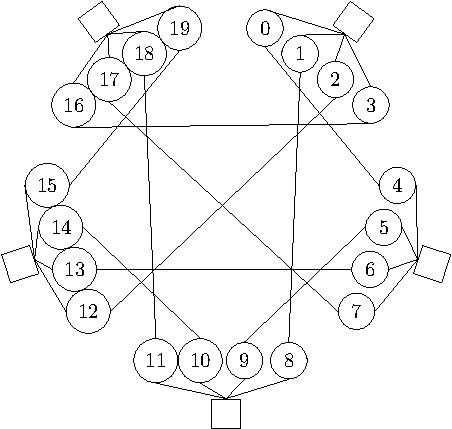
\includegraphics[width=1\textwidth]{figures/topologies/dcell-crop}
        \subcaption{Dcell$_1$ with 4 port switches \cite{GuoWTSZL08}}
    \end{minipage}\hfill
    \begin{minipage}{.95\columnwidth}
        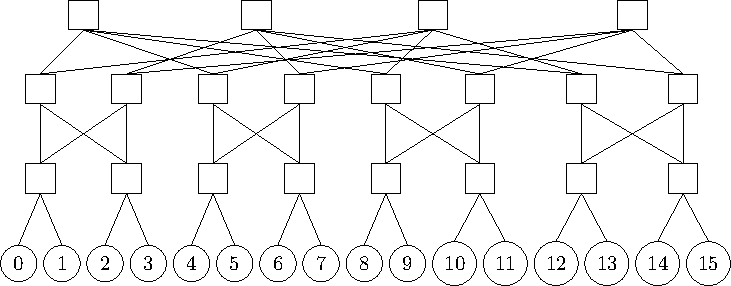
\includegraphics[width=\textwidth]{figures/topologies/fattree}
        \subcaption{Fat Tree with 4 port switches \cite{Al-FaresLV08}}

        \vspace{2.5em}

        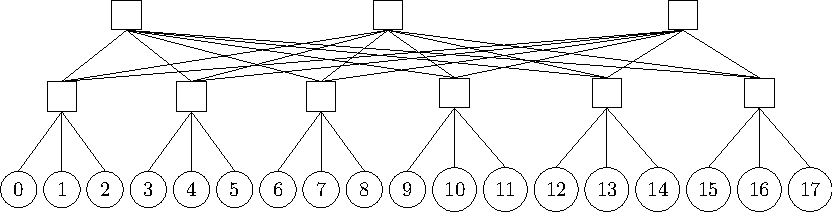
\includegraphics[width=\textwidth]{figures/topologies/leafspine}
        \subcaption{Leaf-Spine with 6 port switches \cite{Cisco19}}
    \end{minipage}\hfill
    \begin{minipage}{.15\columnwidth}
        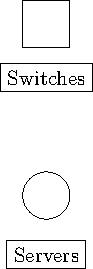
\includegraphics[width=\textwidth]{figures/topologies/key}
    \end{minipage}

    \vspace{1em}
    \caption{Common data center topologies}
    \label{fig:topologies}

	\vspace{1em}
\end{figure*}

\subsubsection{Unrealistic Model}
Other works do consider the QoS but do so in a way that is inconsistent with real world evidence. Most commonly, these works assume that the waiting time at a network component is constant however in practice the waiting time depends on the utilization of the component \cite{IntelDPDK, IntelPPP, OljiraGTB17}.

Many works assume there are constant waiting times at all components in the network. Often, these works use greedy heuristics to solve the simplified problem. For example, Alameddine et al. \cite{AlameddineQA17} proposed greedy, random and tabu heuristics to place VNFs such that tasks are completed before certain deadlines. Vizarreta et al. \cite{VizarretaCMMK17} also assumed constant waiting times but additionally fixed the starting and ending components for each service. They first found the lowest cost route between the starting and ending components that satisfied latency and robustness constraints and then modified the path until it could accommodate each VNF of the service. Qu et al. \cite{QuASK17} used the same assumptions and a similar technique. Their algorithm first attempts to place VNFs on the shortest path between the starting and ending components of each service. If the path cannot accommodate all VNFs then nearby components are also considered.

Other non-greedy heuristics also presuppose constant waiting times. These include Hawilo et al. \cite{HawiloJS19}, who proposed a heuristic named BACON that places latency sensitive VNFs on components with high betweeness centralities and low latency neighbors. Manias et al. \cite{ManiasJHSHLB19} later extended this work, using a decision tree to learn the outputs of BACON. More recently they extended this work to use particle swarm optimization to select the model hyperparameters \cite{ManiasHJS20}. Roy et al. \cite{RoyTSARH20} use ant colony optimization to minimize the overall latency where the ants heuristically favoured nodes with low constant waiting times. Bari et al. \cite{BariCAB15} used dynamic programming to place each service separately aiming to minimize energy and placement costs whilst considering latency constraints.

Using the same constant waiting time assumption, some researchers have combined linear programming with other methods to reduce the number of possibilities the solver must consider. Alleg et al. \cite{AllegKMA17} consider a problem with branching services and used a heuristic to match servers and VNFs by their degree in the network topology and service chain respectively. The solver is then only allowed to place VNFs on those nodes in order to meet latency constraints. Luizelli et al. \cite{LuizelliCBG17} used variable neighborhood search (VNS) to selects subsets of VNFs that can be changed whilst the others variables remain fixed. The new problem is then solved whilst meeting latency constraints using linear programming. A new subset of VNFs are selected for the next iteration and the process is repeated. Pei et al. \cite{PeiHXLWW20} used linear programming to find the exact solution to a set of problems to form a training set and then used supervised learning to learn a model that can place VNFs.

\subsubsection{Ignores Model}
Some researchers recognize the relevance of accurate QoS models but only use it to evaluate the solutions discovered by a heuristic. This provides additional information to the decision maker but does not change the quality of the solutions. Chua et al. \cite{ChuaWZSH16} place VNFs of each service in the first server that can accommodate it, but restrict the maximum capacity of each server until all available capacity has been used. They then use an queueing model to inform the end user of the expected latency. Similarly, Zhang et al. \cite{ZhangXLLGW17} propose a best fit decreasing method of placing VNFs and use an queueing model to evaluate the solution.

\subsection{Realistic and Scalable}
Finally, there are some works that meet both of the main criteria but which may be improved upon. Some works use more accurate but still imperfect models with known issues. For example, several works disregard packet loss when constructing their model. Whilst this greatly simplifies the model construction it also misrepresents the problem as packet loss impacts on service latency and energy consumption \cite{BillingsleyLMMG22}. Gouareb \cite{GouarebFA18} et al. use this type of model to calculate the latency, and present linear programming and heuristic solutions that minimize the latency. The heuristic greedily assigns VNFs with the largest requirements to the server with the most capacity and then scales VNFs horizontally (more instances) or vertically (more resources per VNF) to meet demand. Leivadeas et al. \cite{LeivadeasFLIK18} use the same form of model with Tabu search to jointly minimize energy and latency. Qu et al. \cite{QuZYSLR20} use the same model to minimize cost whilst considering latency constraints. They propose a heuristic that attempts to reallocate resources on overloaded nodes to services which are violating constraints and if necessary to migrate services so as to avoid overloaded nodes.

In our earlier work on this problem \cite{BillingsleyLMMG20}, we proposed a routing-led multi-objective genetic algorithm that used an accurate queueing model of a data center. This earlier work could scale to problems with up to $\sim$16,000 servers. On larger problems, the time and memory requirements of the algorithm are impractical.

% \subsection{Conclusion}
% From the literature review we can see that the majority of works are impractical as they are either unable to scale to large problems or are solving overly simplified problems that do not reflect the real world. The remaining works typically rely on unverified models that may or may not be suitable. In this work, we propose a scalable solution that solves a realistic reflection of the problem. Further, we determine whether the alternative models used in some scalable solutions are suitable.